%!TEX root = main.tex
\section{The Sensemaking Model for VQSs\label{sec:sensemaking}}
\change{
  To convey how the features in \zvpp addresses the analytical needs posed by each domain, we organize our PD findings into a sensemaking framework for VQSs. In this section, we first describe the space of problems addressable by VQSs. Then, as shown in Figure~\ref{fig:taxonomy}, we develop a taxonomy for organizing VQS functionalities into three sensemaking processes. From top to bottom, we first describe the design objectives of each sensemaking process, then we outline the design challenge addressed by each of the functional components that supports the sensemaking process. The mapping between specific \zvpp features and these functional components and sensemaking processes can be found in Table~\ref{bigfeaturetable}.
}
 %Starting from the bottom level of the taxonomy, we first describe what each component in our taxonomy encompasses, then we proceed onto the upper level of the taxonomy, .
%We first describe features that we incorporated into our enhanced VQS, \zvpp, thematically organized by components (grouping features in the bottom-most level to components in the second level of Figure~\ref{fig:taxonomy}).
%collaboratively-designed
%Next, we describe features that we incorporated into our enhanced VQS, \zvpp, thematically organized by component. Then, we introduce a taxonomy for organizing these components into three sensemaking processes, spanning different problem areas that VQSs are aimed to solve.
%\change{In this section, we will first introduce a taxonomy for organizing these components into}
%Based on feature requests and discussion with our participants, we incorporated key features missing in our original VQS.
%From these discussion and analysis of past VQSs, we identify nine components of VQSs, described below. T
% Along with analysis of past literature, we develop a taxonomy of key functionalities in VQSs.
% novel contribution on  ---
% contribute to holistic understanding on how sensemaking --- in VQS.
% study on how users
% Implication ---
% •	What types of questions/ dataset/ problem challenges are asked to VQS or can be addressed by VQS? (S3)
% •	What kind of features needs to be designed to address these challenges (S4 PD)
%We employed participatory design with our scientists to incorporate key features missing in our original VQS, and unaddressed in their existing workflows. From these discussion and analysis of past VQSs, we identify nine components of VQSs, described below.
\begin{figure*}[ht!]
  \centering
  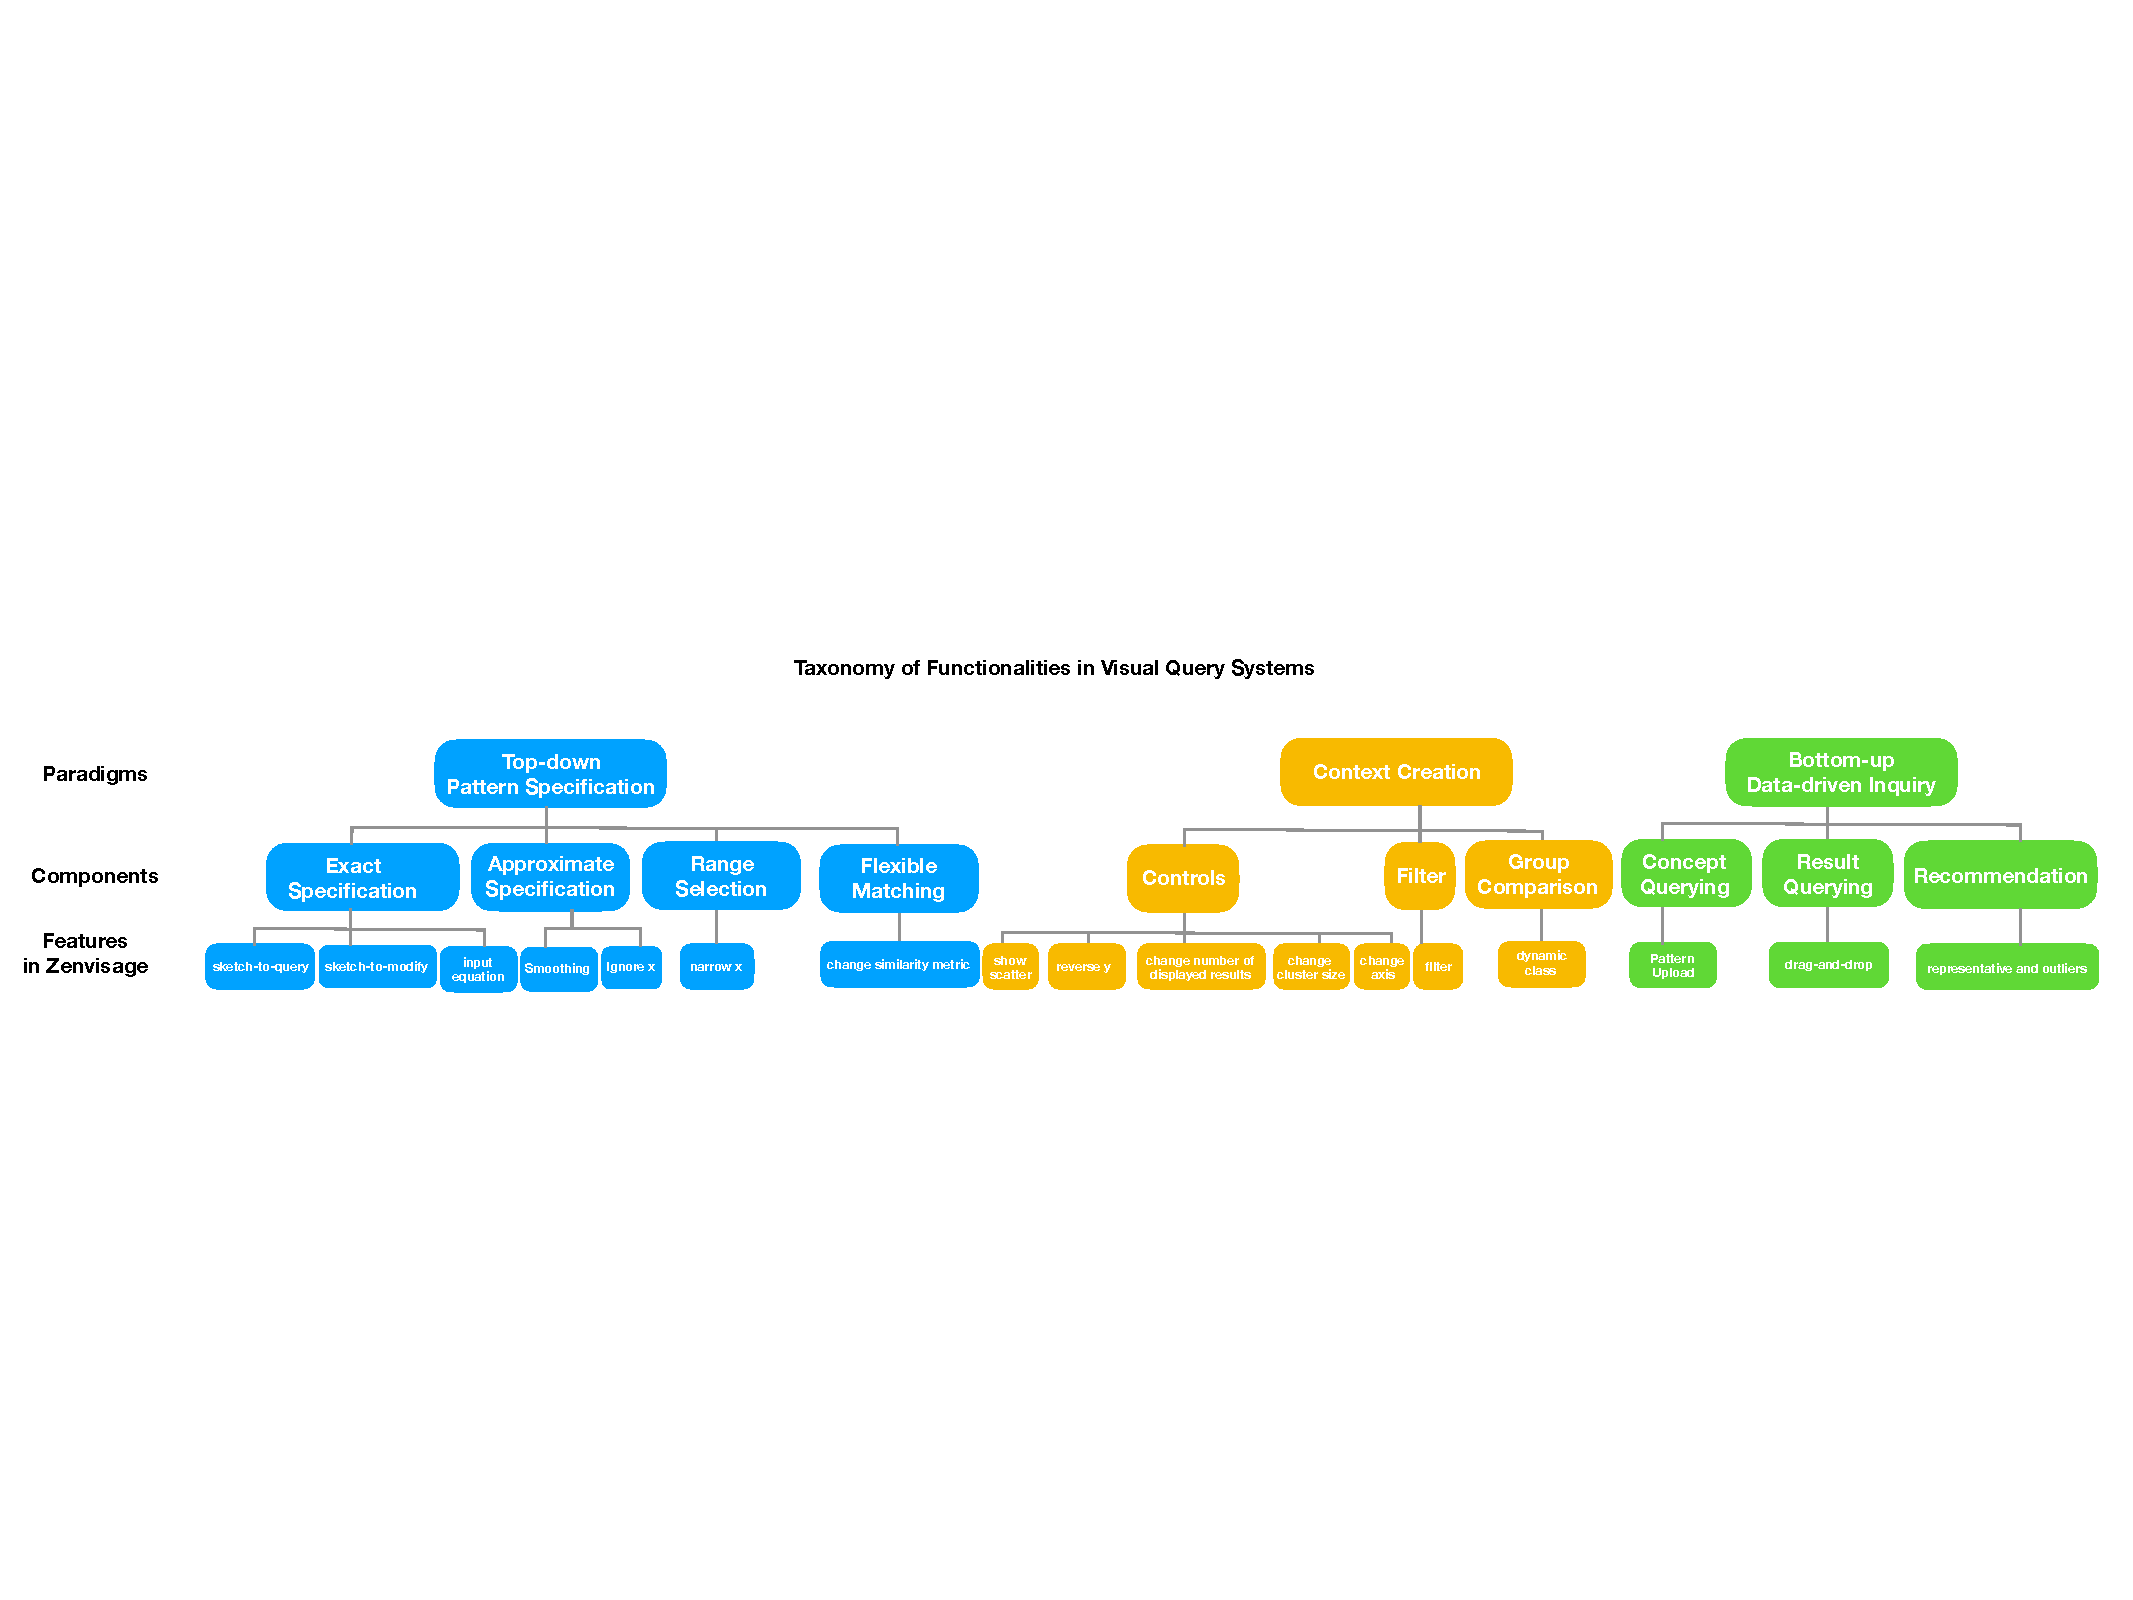
\includegraphics[width=0.9\linewidth]{figures/taxonomy.pdf}
  \caption{Taxonomy of functionalities in VQSs. Each of the three sensemaking process is broken down into key functional components in VQSs. \change{We list the types of questions addressed by each component from a system's perspective.}} %, which is instantiated as features in \zvpp.}% The bottom-most layer connects the use cases features that have practical or envisioned usage based on the evaluation study.}
  \label{fig:taxonomy}
\end{figure*}
\subsection{Characterizing the Problem Space for VQSs}
%Based on example use cases and feature components from participatory design, we further characterize the design space of VQSs. further characterize three sensemaking process within the problem space of VQSs.
%Given our earlier description of VQS features organized into components, we
\change{We now} introduce the three sensemaking processes by characterizing how they fit into different problem areas that VQSs are aimed to solve. Visual querying often consists of searching for a desired pattern instance (Z) across a visualization collection specified by some given attributes (X,Y). \change{Correspondingly, }we introduce two axes depicting the amount of information known about the visualized attribute and pattern instance.%, as shown in Figure~\ref{2dmodel}.
%(e.g., only interested in patterns related to a specific gene)
\par Along the \textbf{pattern instance} axis,
the visualization that contains
the desired pattern may already be \texttt{known} to the analyst,
exist as a pattern \texttt{in-the-head} of the analyst,
or completely \texttt{unknown} to the analyst.
In the \texttt{known} pattern instance region (Figure~\ref{2dmodel} grey), visualization-at-a-time systems such as Tableau,
where analyst manually create and examine each visualization one at a time,
is more well-suited than VQSs, since analysts can directly work with the selected instance without the need for visual querying.
Inspired by Pirolli and Card's information
foraging framework~\cite{Pirolli}, which distinguishes
between information processing tasks that are \textit{top-down}
(from theory to data) and \textit{bottom-up} (from data to theory),
we define \textit{top-down pattern specification} as the search-oriented paradigm where analysts query based on their
in-the-head pattern (Figure~\ref{2dmodel} blue) in a fixed collection.
On the other hand, in the realm of \textit{bottom-up
data-driven inquiry} (Figure~\ref{2dmodel} green),
the pattern of interest is unknown\change{, external
to the user, }and must be driven by recommendations
or queries that originate from the data (or equivalently, the visualization).
As we will discuss later, this process is crucial
but underexplored in past work on VQSs.
%analysts often do not start with a known pattern instance. T
\par The second axis, \textbf{visualized attributes},
depicts how much the analyst
knows about which X and Y axes
they are interested in visualizing.
In both the astronomy and genetics use cases,
as well as past work in this space,
data was in the form of a time series
with \texttt{known} visualized attributes.
In the case of our material science participants,
they wanted to explore relationships between different
X and Y variables.
In this realm of \texttt{unknown} attributes,
context creation (Figure~\ref{2dmodel} yellow) is
essential for allowing users
to pivot across different visualization collections.%subspaces. %Most past VQSs assume that the analyst has a desired pattern in-the-head that could be conveyed through visual specification, such as a sketch.%---i.e., setting the stage for bottom-up or top-down processes---\dor{this clause is awkward?}
\begin{figure}[h!]
  \centering
  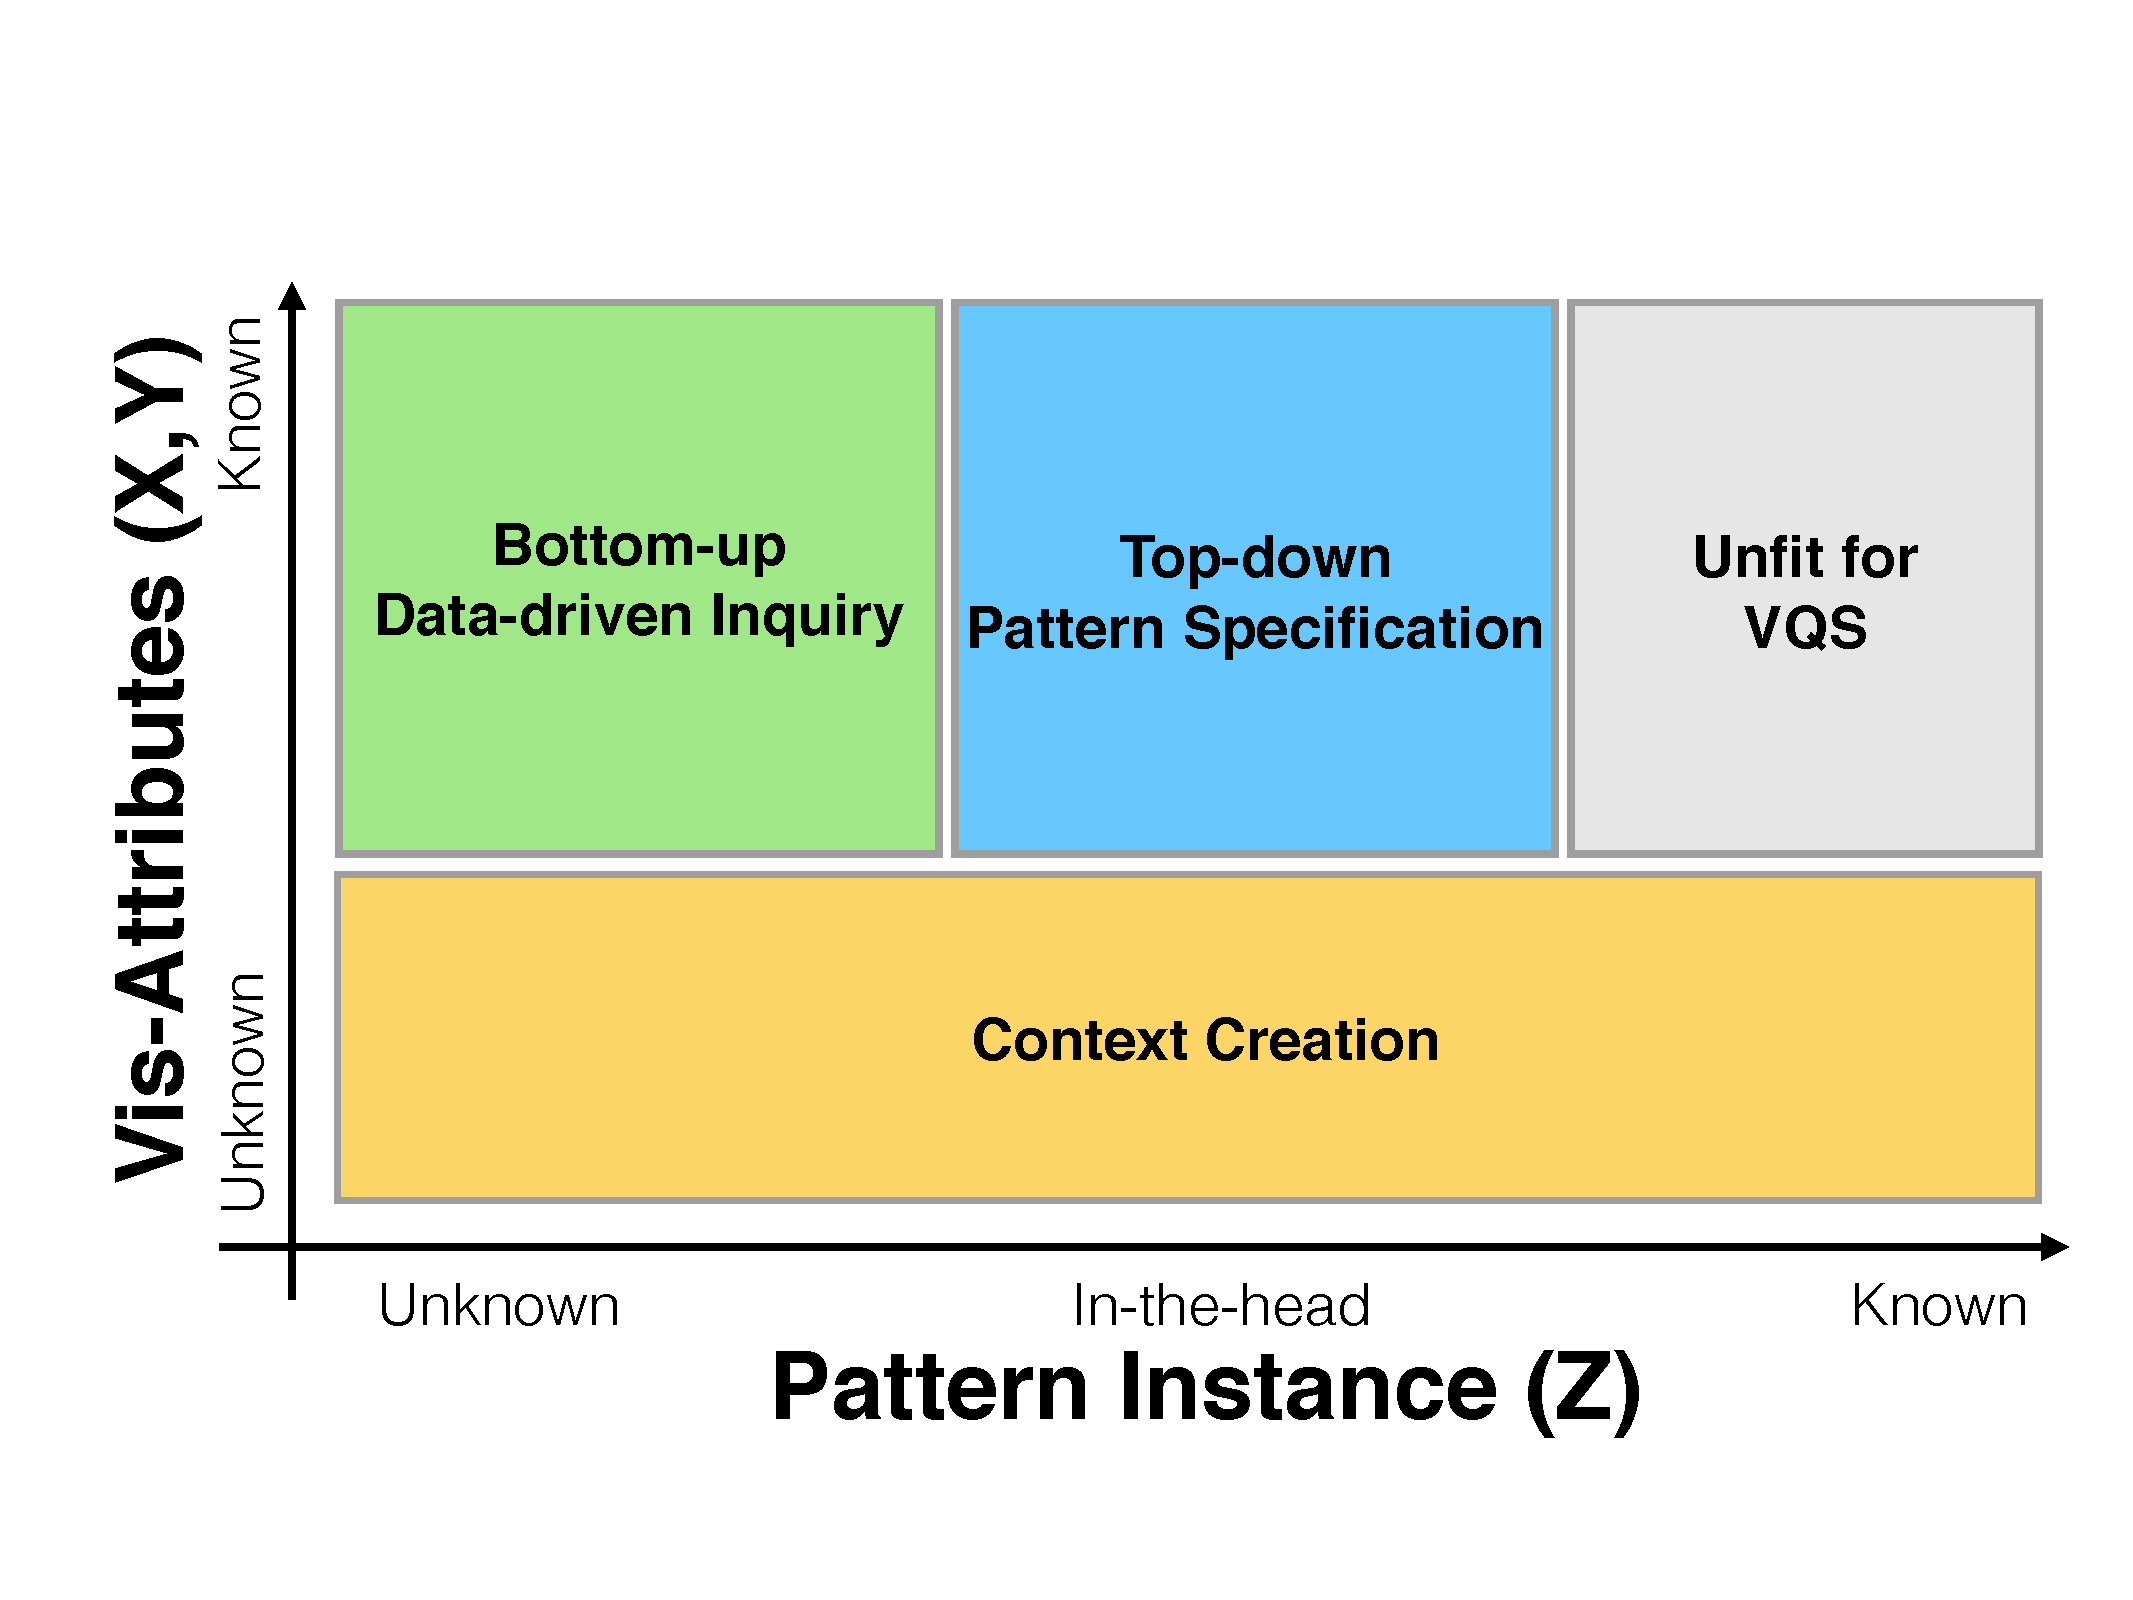
\includegraphics[width=0.9\linewidth]{figures/2dmodel.pdf}
  \caption{The problem space for VQSs is characterized by how much the analyst knows about the visualized attributes and the pattern instance. Colored areas highlight the three sensemaking processes in VQSs for addressing these characteristic problems. While prior work has focused solely on use cases in the blue region, we envision opportunities for VQSs beyond this to a larger space of use cases covered by the yellow and green regions.}
  \label{2dmodel}
  \vspace{-10pt}
\end{figure}
\subsection{Design Goals for the Sensemaking Processes}
After understanding how each sensemaking process fits into the problem space \change{addressable} by VQSs, we further explore the design objectives and challenges in supporting each sensemaking process, grounded in our collaborative design experience. % based on the taxonomy orgaby developing a taxonomy for organizing the aforementioned components.% fits into the paradigms of sensemaking in VQSs, as shown in Figure~\ref{fig:taxonomy}. In particular, we will describe the main form of inquiry addressed by each paradigm\cut{(\textit{what, where, which})}, its characteristic use case, and design challenges in supporting these paradigms.
% \par Drawing from our participatory design experience, evaluation study, and literature review in this space, we design a taxonomy for understanding the key functionalities in VQSs. In Figure~\ref{fig:taxonomy}, we show how each use cases makes use of the different features in \zv, then we organize the features into key components for VQSs, which belongs to one of the three paradigms in the VQS design space.%, effectively moving rightwards to the gray area in Figure~\ref{2dmodel}, where the pattern instance is known.
\boldpara{Top-down Pattern Specification} begins with the user's intuition
about how their desired patterns should look like based on `theory', including visualizations from past experience or abstract conceptions based on external knowledge. The goal of top-down pattern specification is to address the \textit{which} question of visual sensemaking: \textit{which pattern instance exhibits this pattern?} Based on this preconceived notion of what to search for, the design challenge is to translate the query in the
analyst's head to a query executable by the VQS.
\change{In the Figure~\ref{fig:taxonomy} taxonomy},
this includes both components for specifying the pattern,
as well as controls governing the underlying
algorithm of how shape-matching is performed.
For example, A1 knows intuitively
what a supernovae pattern looks like
and the detailed constraints on the shape,
such as the width and height of the peak
or the level of error tolerance for defining a match.
He can search for transient patterns through sketching,
select the option to ignore differences
on the x axis, and changes the similarity metric for flexible matching.  %The design challenge of top-down pattern specification is to ----- enable users to How to translate the in-the-head query to visual query and how matching is done.
\boldpara{Bottom-up data-driven inquiry} is
a browsing-oriented sensemaking process
that goes from data to theory to
addresses the \textit{what} questions
in the sensemaking process.
% While the usage of each querying feature may vary from one participant to the next, generally, result querying and pattern upload are considered bottom-up approaches that go from data to theory by enabling users to query via examples of known visualizations. Bottom-up data-driven inquiries
 For example, genetics participants do not
 have a preconceived knowledge of what to search
 for in the dataset.
 They were mostly interested in
 \textit{what types of patterns exist in the dataset}
 through representative trends, as a means to
 jumpstart further queries. %The goal of data-driven inquiry is to move towards the blue area in Figure~\ref{2dmodel} to help analysts gain more information about patterns of interest in-the-head.
% notion of what the pattern looks like
The design challenge include developing
the right set of `stimuli' that could
provoke further data-driven inquiries,
as well as low-effort mechanisms to search via these results.
\boldpara{Context Creation} addresses the \textit{where}
question of sensemaking by enabling analysts
to navigate across different parts of the visualization
collection to learn about \textit{where \change{in the dataset do} the patterns of interest lie}.
For example, material scientists often do not start
with a pattern in-the-head, but recognize salient
trends such as inverse correlation or linear correlation.
They switch between different visualized attributes or dynamic
classes to study their data from alternative perspectives.
The design challenge of context creation is to develop
features that act as a `lens': navigating users to desired data subsets,
visualizing and comparing how the data changes between the different lenses, and ensuring that context is dynamically reflected across other VQS functionalities.
\par\noindent The three aforementioned sensemaking processes are akin to the well-studied sensemaking paradigms of search, browse, and faceted navigation on the Web~\cite{Hearst2009,Olston2003}. Due to each of their advantages and limitations given different information seeking tasks, search interfaces have been designed to support all three complementary acts and transition smoothly between them to combine the strength of all three paradigms. \change{Similarly for VQSs, our main design objective in developing \zvpp is to integrate all the three sensemaking in the same system. As we discover in the evaluation study in the following section, this integration encourages and accelerates the process of visualization discovery.}
\change{
  \subsection{Functional Components of VQSs\label{sec:component}}
    Here, we discuss the motivation for each functional component in the lower-level of our Figure~\ref{fig:taxonomy} taxonomy and how they address specific challenges posed by the problem and dataset characteristics from each domain.
    \boldpara{Pattern Specification} interfaces allow users to submit exact descriptions of a pattern query with the VQS returning a list of most similar matches. This is useful when the dataset contains \emph{large numbers of potentially-relevant pattern instance}.
    Since it is often difficult to sketch precisely, additional characteristics of the pattern query (e.g., pattern query expressible in a functional form, or has specific shape characteristics) can be used to further winnow the list of undesired matches.
    \boldpara{Match Specification} addresses the well-known problem in VQSs where pattern queries are imprecise~\cite{correll2016semantics,Holz2009,Eichmann2015} by allowing users to clarifying how matching should be performed.
    Match specification is useful when the dataset is \emph{noisy} (i.e., containing large numbers of false-positives that could be matched). When the pattern query satisfies some additional constraints, adjusting match specification to prune away these false-positives help reveal true candidates.
    \boldpara{View specification} settings alter the specifications for all of the candidate visualizations being explored on the VQS. The ability to work with different collections of visualizations is useful when the dataset is \emph{multidimensional} and the axes of interest is \emph{unknown}. Modifying the view specification offers analysts different perspectives on the data to locate visualization collections of interest.
    \boldpara{Slice-and-Dice} empowers users to navigate and compare different collections of visualizations constructed from different portions of the data. Slice-and-dice is useful when the dataset has \emph{large numbers of non-visualized attributes} that may be related to the visualized attributes (e.g., geographical location may influence the time series pattern for housing prices). Analysts can either make use of pre-existing knowledge regarding these `support' attributes to navigate to a data region that is more likely to contain the desired pattern (e.g., filtering to popular cities such as New York to find expensive houses) or discover unknown patterns and relationships between different data subsets (e.g., housing prices is lower around winter than compared to summer).% by gaining a better understanding of characteristic patterns in particular data region.
    \boldpara{Result querying} allows users to submit a query based on the results, essentially asking for patterns similar to the selected data pattern. Typically, analyst associate selected visualizations with some \emph{semantic or visual properties} and make use of results querying to understand characteristic properties of similar instances.
    \boldpara{Recommendation} displays visualizations that may be of interest to users based on the data context. Representative trends and outliers are useful when a \emph{small number of common patterns} is exhibited in the dataset. Understanding \emph{characteristic} patterns in dataset can help analysts discover other pattern queries of interest to jumpstart further queries.
  % % In this section, we first describe a model to help characterize the design space for VQS based on the analytical workload and usage patterns from different use cases. Then, we present design challenges related to each of the process.
}
